\newpage
\chapter{Обучение на мрежата}
\label{chapter07}

Обучението при класическите многослойни изкуствени невронни мрежи е свързано с оптимизация на теглата, които характеризират връзките между отделните неврони. По своята същност задачата за обучение представлява числена оптимизация в многомерно пространство на реалните числа. През последните няколко десетилетия са разработени множество точни числени методи и множество евристични методи. В настоящата разработка акцентът пада над два метода (единият точен числен, а другият евристичен). Като точен числен метод софтуерната библиотека Encog предлага широко използваният метод с обратно разпространение на грешката (както и някои негови модификации). От групата на евристичните методи се използват генетични алгоритми с модификация на мутацията, според метода за еволюция на разликите. За реализацията на генетичния алгоритъм се използва софтуерната библиотека Genetic Algorithms - Apache Commons.

\section{Обратно разпространение на грешката}

При обратното разпространение на грешката, в работен режим, сигналите пътуват от входа на мрежата към нейния изход. Тренировъчните примери се прилагат в случайно определен ред, така че мрежата да не заучи схемата на подаване, а да развие своите обобщаващи способности. Общата допусната грешка се изчислява на изхода на мрежата и след това се връща по обратния път, от изход към вход, за да бъде изчислена грешката с която всеки неврон допринася. След определянето на индивидуалната грешка за всеки неврон се извършва числена корекция (според градиента) на теглата, които свърват невроните. Този обратен ход на пресмятане дава името на метода и също така го поставя в групата на точните числени методи, които разчитат на градиента за да извършат корекция в теглата. Същественото за обучението с обратно разпространение на грешката е, че активационната функция на неврона трябва да бъде диференцируема. Библиотеката Encog предлага серия методи за корекция на теглата в мрежата. 

\begin{figure}[h]
  \centering
  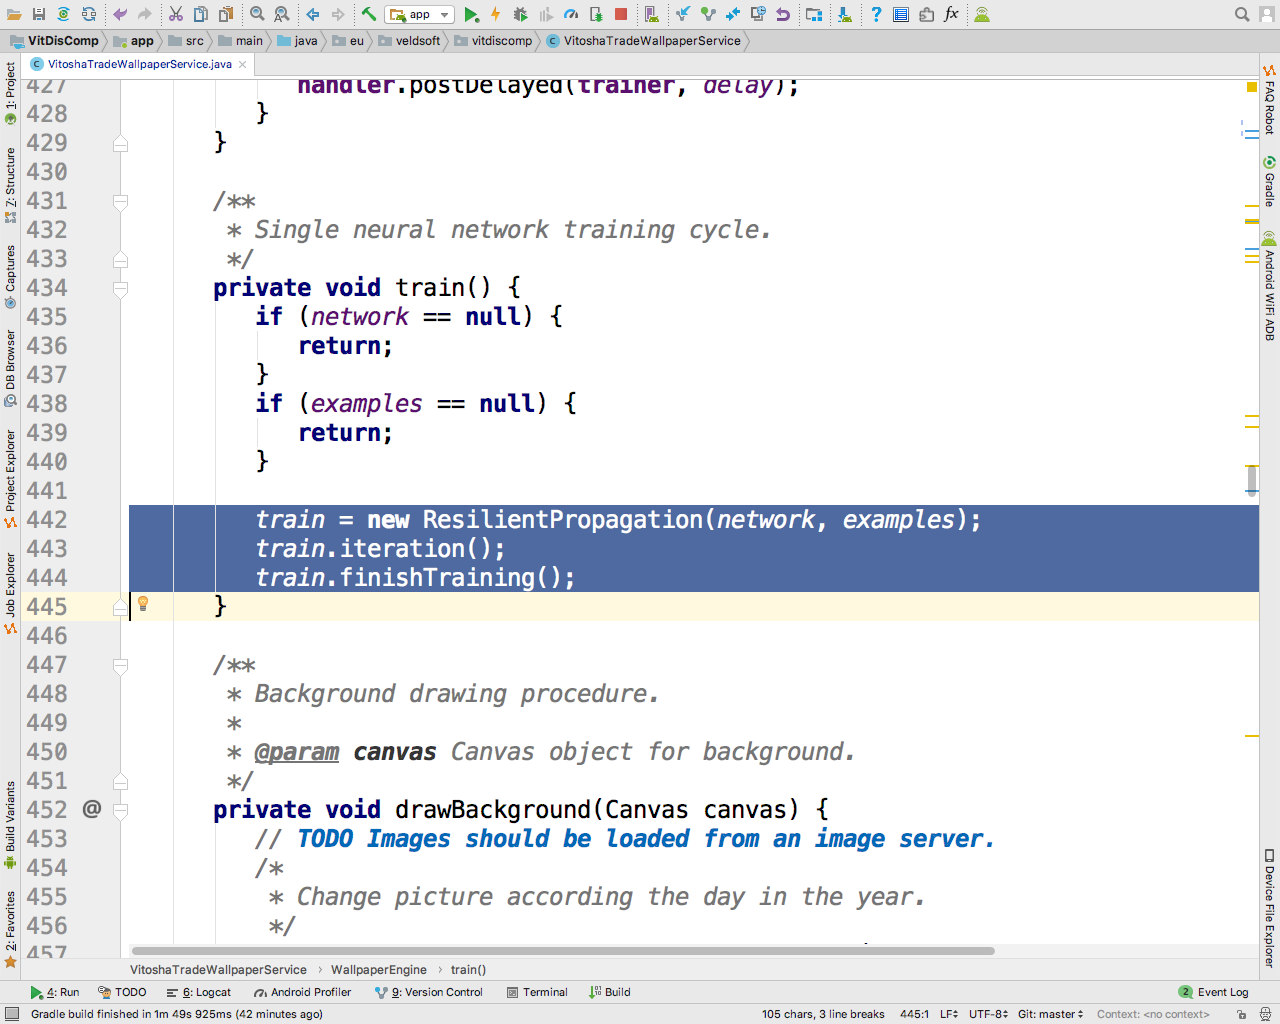
\includegraphics[height=0.45\pdfpageheight]{pic0173}
  \caption{Единична стъпка за обучение на мрежата.}
\label{fig:pic0173}
\end{figure}
\FloatBarrier

Библиотеката Encog позволява няколко възможности за обучение с точни числени методи и в настоящата разработка е избран метода Resilient Propagation, който представлява еластично обратно разпространение на грешката (Фиг. \ref{fig:pic0173}). Еластичното разпространение на грешката е модификация на основния метод в която модификация степента за научаване (learning rate) се определя динамично и не е само една стойност за цялата мрежа. При класическия подход с обратно разпространение на грешката степента за научаване е само една стойност, обикновено емпирично нагласена между 0.0 и 1.0. Най-често се използва 0.35, което е компромис между бързината за научаване и достигането на оптимална стойност за теглата (фината стъпка за нагласяне на телата в крайната фаза от обучението).

\begin{figure}[h]
  \centering
  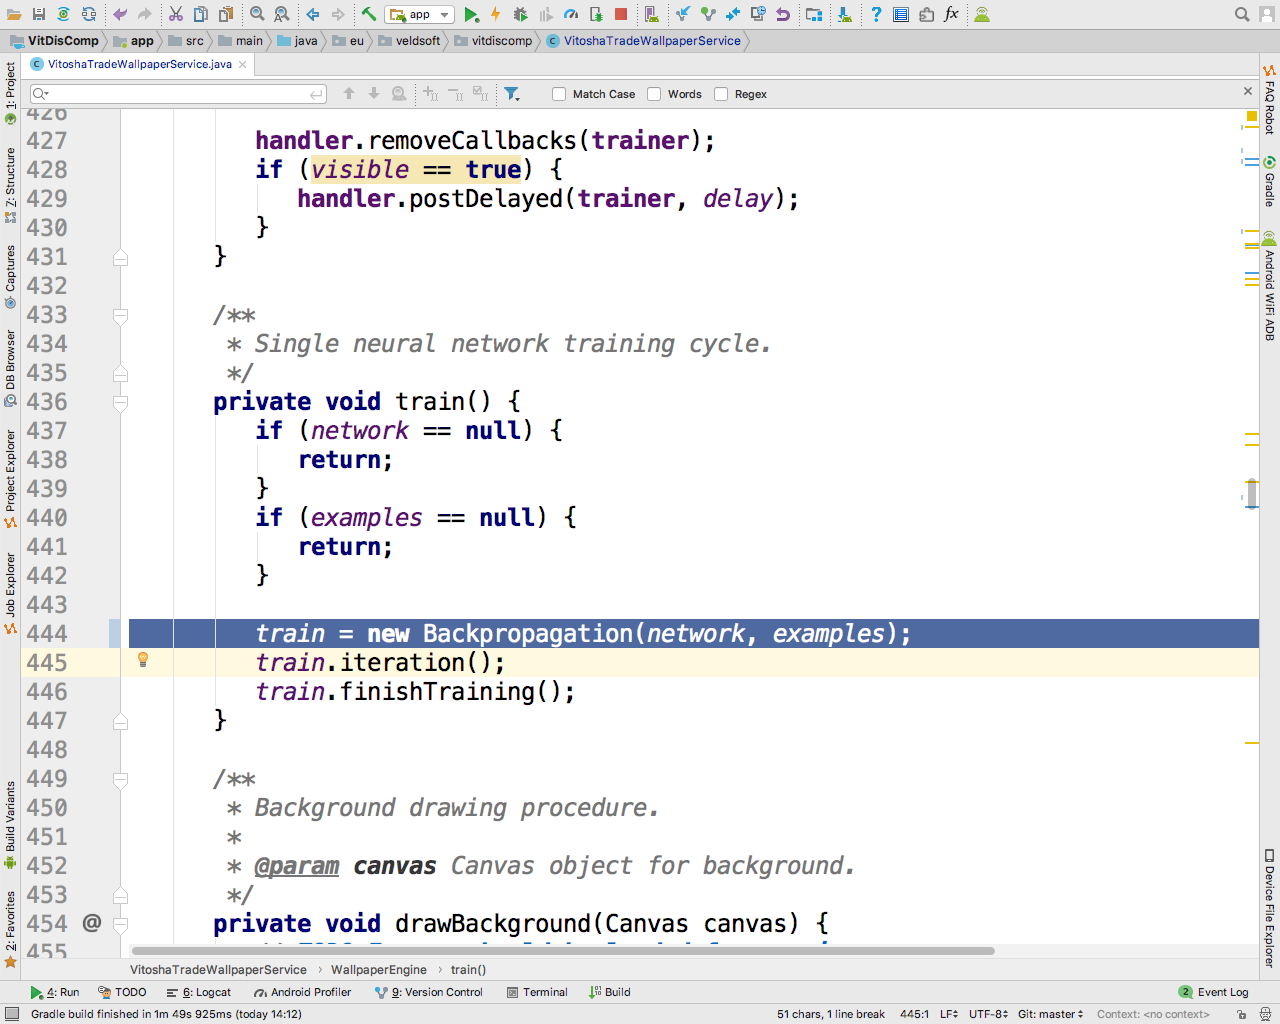
\includegraphics[height=0.45\pdfpageheight]{pic0174}
  \caption{Класическо обратно разпространение на грешката.}
\label{fig:pic0174}
\end{figure}
\FloatBarrier

Фактът, че библиотеката Encog е написана по каноните на обектно-ориентираното програмиране, позволява само с подмяната на един ред (Фиг. \ref{fig:pic0174}) от еластично обучение да преминем към класическо обратно разпространение на грешката. 

\begin{figure}[h]
  \centering
  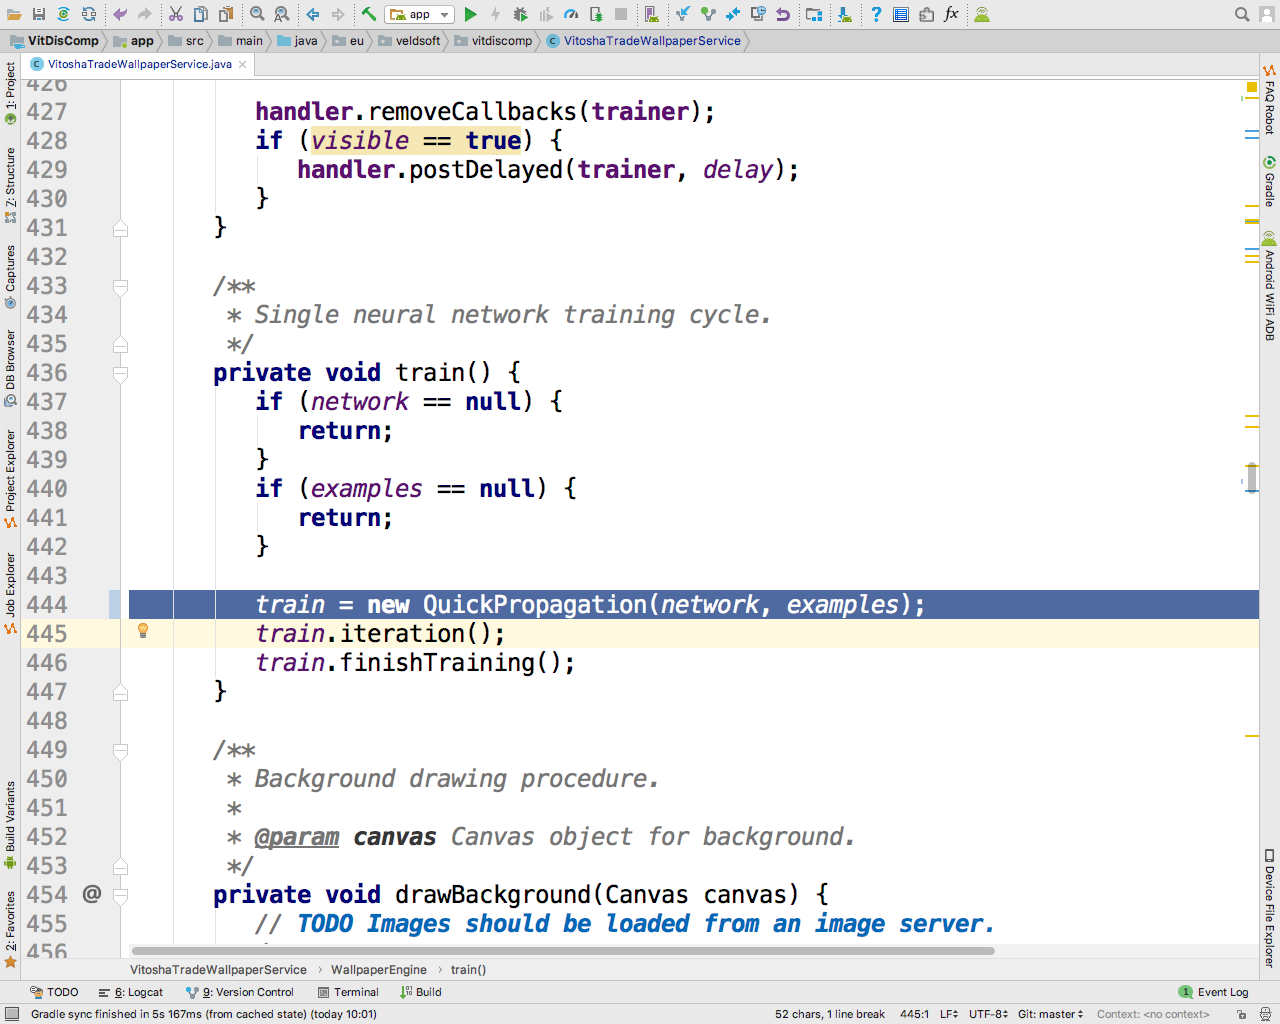
\includegraphics[height=0.45\pdfpageheight]{pic0175}
  \caption{Бързо разпространение на грешката.}
\label{fig:pic0175}
\end{figure}
\FloatBarrier

С абсолютно същата лекота, библиотеката позволява да се премине към бързо разпространение на грешката (Фиг. \ref{fig:pic0175}). Тази модификация на алгоритъма за обратно разпространение на грешката въвежда подобрение, чрез използването на метода Нютон-Равсън за допълнително определяне на втората производна, така че допълнителната информация от втората производна да подобри начина по който се коригират теглата в мрежата. Благодарение на тази модификация, по наклоните на функцията за грешка с правят по-големи стъпки, а при доближаване на екстремалната точка стъпката се намалява. 

\begin{figure}[h]
  \centering
  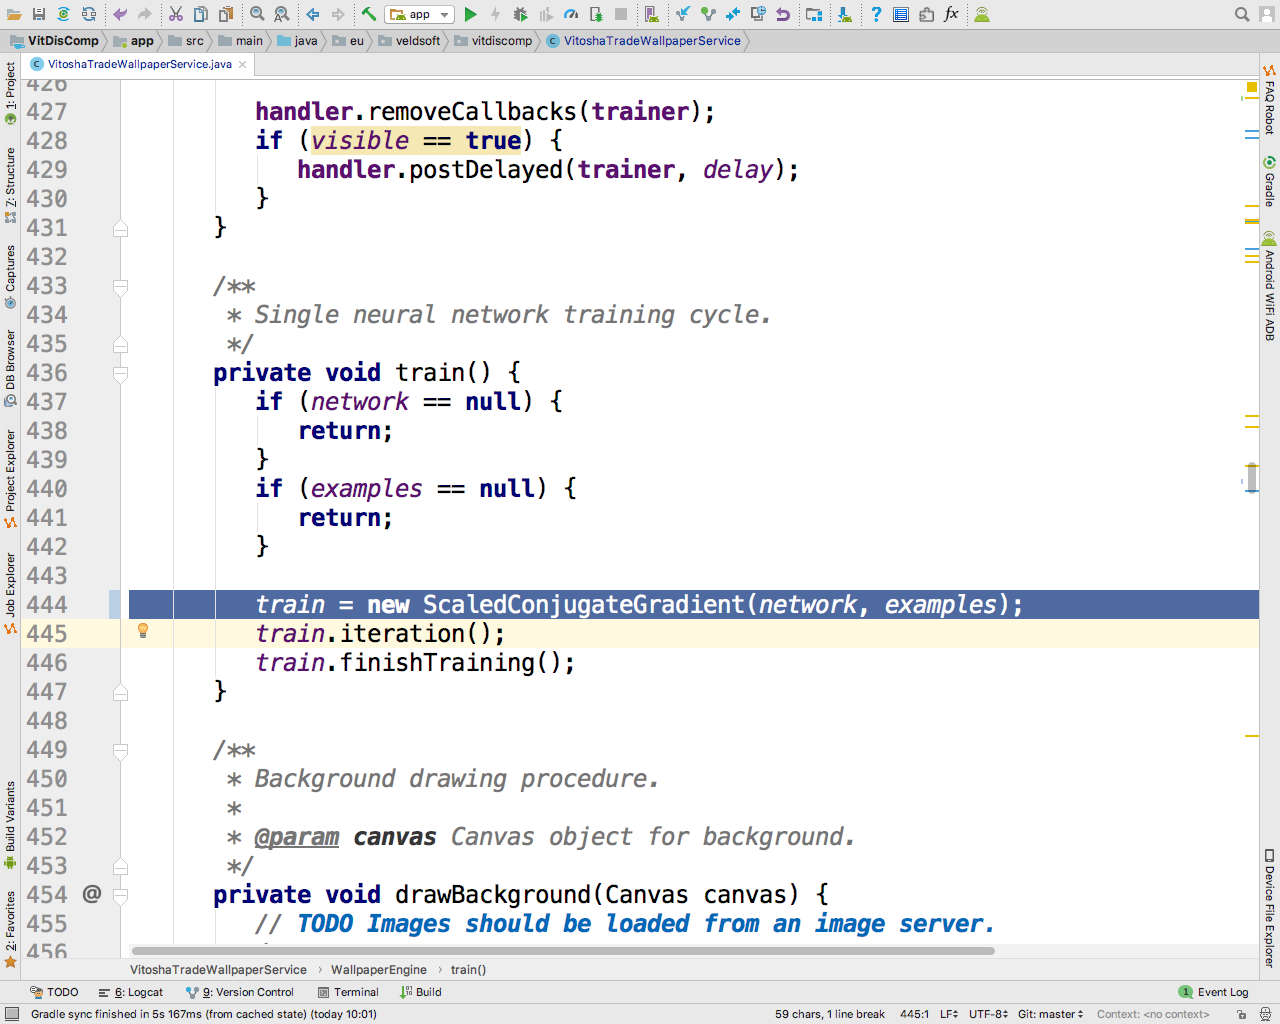
\includegraphics[height=0.45\pdfpageheight]{pic0176}
  \caption{Мащабирано съединение на градиента.}
\label{fig:pic0176}
\end{figure}
\FloatBarrier

При мащабираното съединение на градиента (Фиг. \ref{fig:pic0176}) също се използва информацията от втората производна. По този начин се намира по-добър път към оптималната точка в сравнение с методите, които използват само първа производна. Цената на такова подобрение е нуждата от използването на повече изчислителни ресурси. Разликата при този метод е, че корекцията на теглата не винаги са в посоката посочена от първата производна. 

\begin{figure}[h]
  \centering
  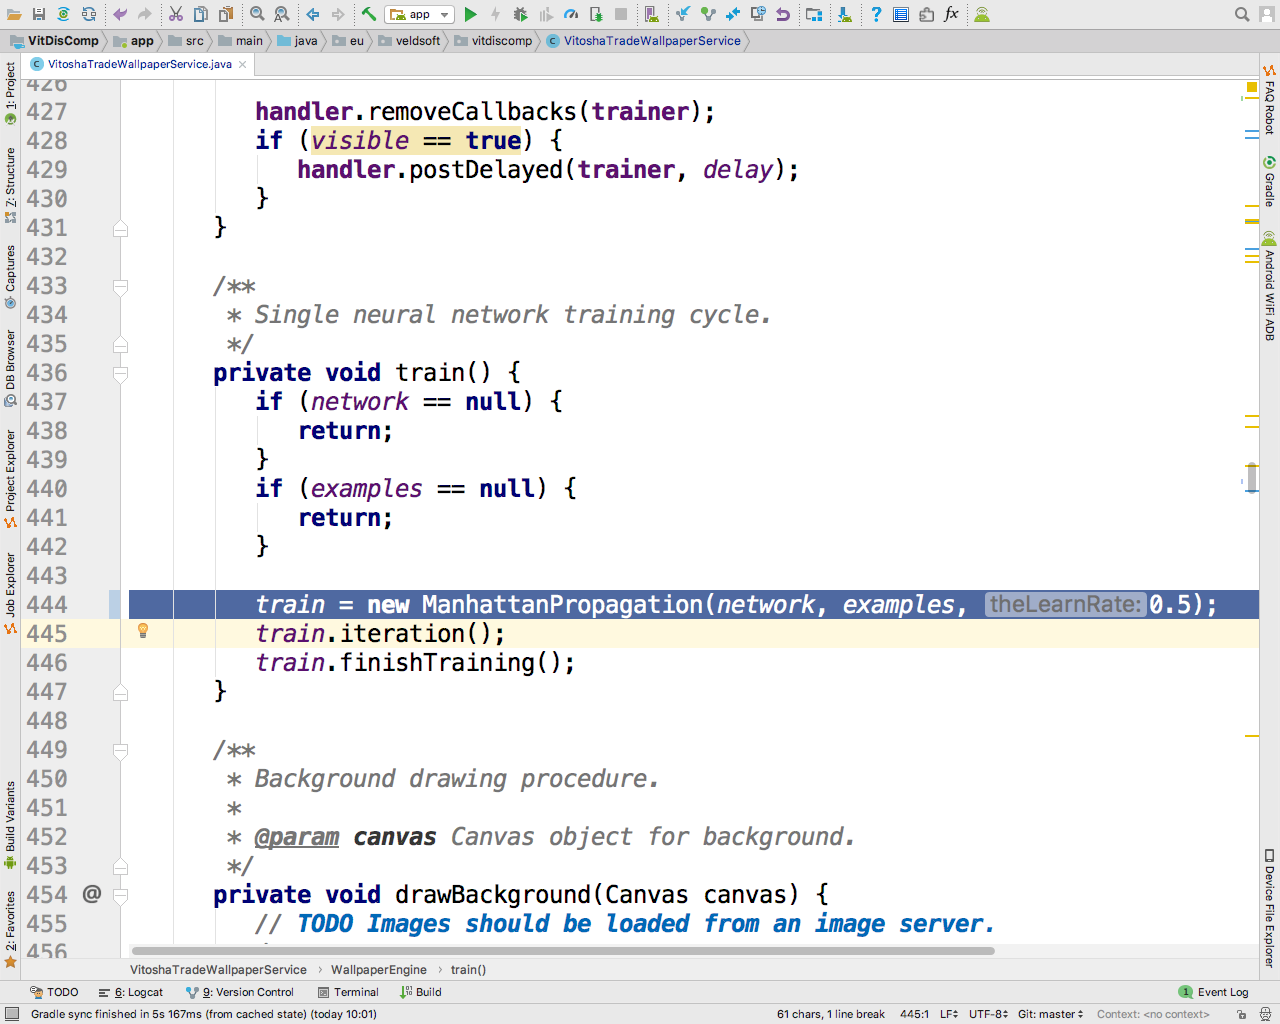
\includegraphics[height=0.45\pdfpageheight]{pic0177}
  \caption{Корекция на теглата по Манхатън правило.}
\label{fig:pic0177}
\end{figure}
\FloatBarrier

Опростен вариант на еластичното обучение е корекцията на теглата по Манхатън правило (Фиг. \ref{fig:pic0177}). При тази модификация на обратното разпространение на грешката се използва само посоката на първата производна, като за корекция на теглата се прилага единична, предварително дефинирана стойност (theLearningRate). При този метод ползата идва от това, че понякога първата производна се пресмята до твърде голяма или твърде малка стойност. Когато корекцията е с фиксирана стойност и се използва само посоката на производната се избягва негативния ефект на големи/малки стойности за корекция. Недостатък на този алгоритъм е, че единичната стойност за корекция трябва да бъде адаптивно нагласяна. Обикновено се започва с по-голяма стойност и се намалява, по аналогия с метода за симулирано закаляване. 

\section{Генетични алгоритми}

Въпреки че библиотеката Encog има възможности за обучение на изкуствени невронни мрежи с генетични алгоритми (класът MLMethodGeneticAlgorithm) в настоящата разработка е предпочетена библиотеката Genetic Algorithms - Apache Commons, тъй като тя дава много повече свобода за реализация на операциите в генетичния алгоритъм и разширения в посока на метода за еволюция на разликите. 

\begin{figure}[h]
  \centering
  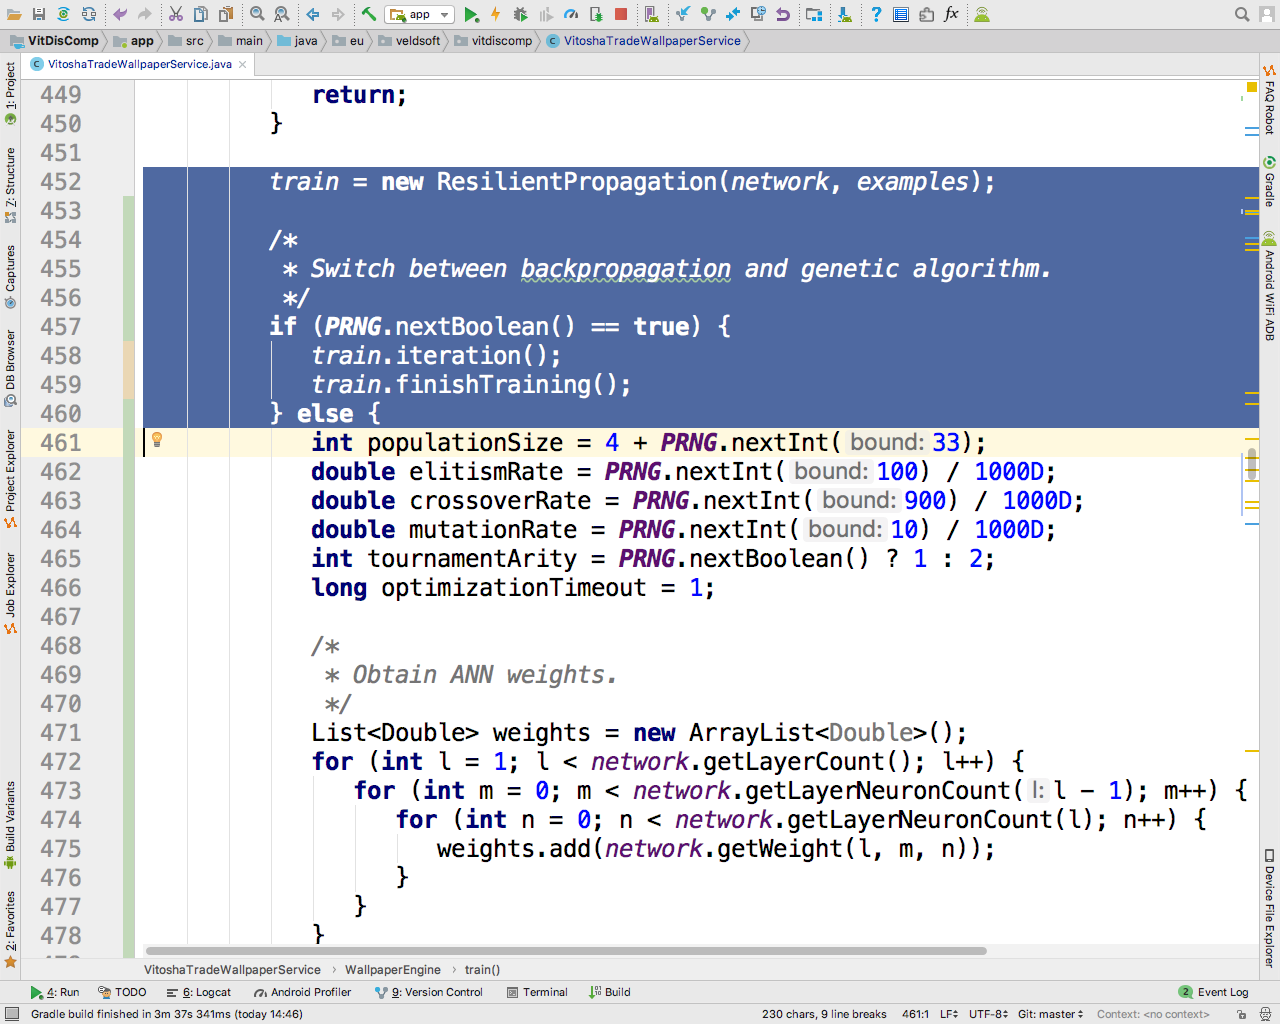
\includegraphics[height=0.45\pdfpageheight]{pic0178}
  \caption{Превключване между ОРГ и ГА.}
\label{fig:pic0178}
\end{figure}
\FloatBarrier

С добавянето на генетичен алгоритъм се получава хибридна система за обучение на изкуствени невронни мрежи (Фиг. \ref{fig:pic0178}). На случаен принцип, в половината от случаите се извършва обучение с точен числен метод, а в другата половина с евристичен метод. 

\begin{figure}[h]
  \centering
  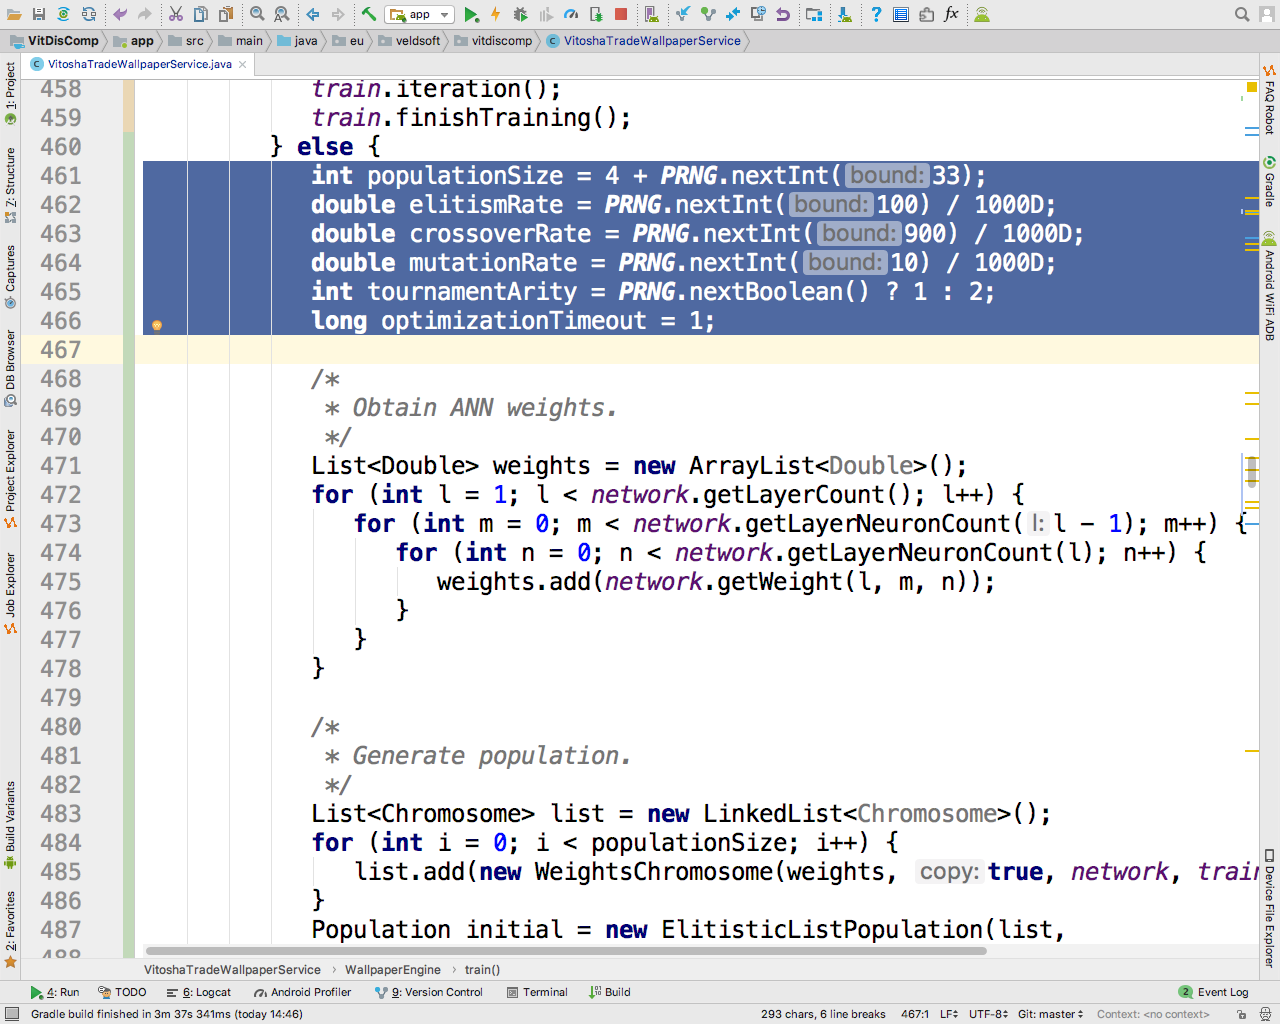
\includegraphics[height=0.45\pdfpageheight]{pic0179}
  \caption{Параметри на генетичния алгоритъм.}
\label{fig:pic0179}
\end{figure}
\FloatBarrier

Генетичният алгоритъм се настройва с група параметри (размер на популацията, процент на елита в популацията, честота за кръстосване, честота за мутация, численост за турнамента при селекция и максимален брой секунди за извършване на оптимизация), които в случая са статично зададени, но е разумно да бъдат управлявани от конфигурационен файл или от екран за настройки (Фиг. \ref{fig:pic0179}). 

\begin{figure}[h]
  \centering
  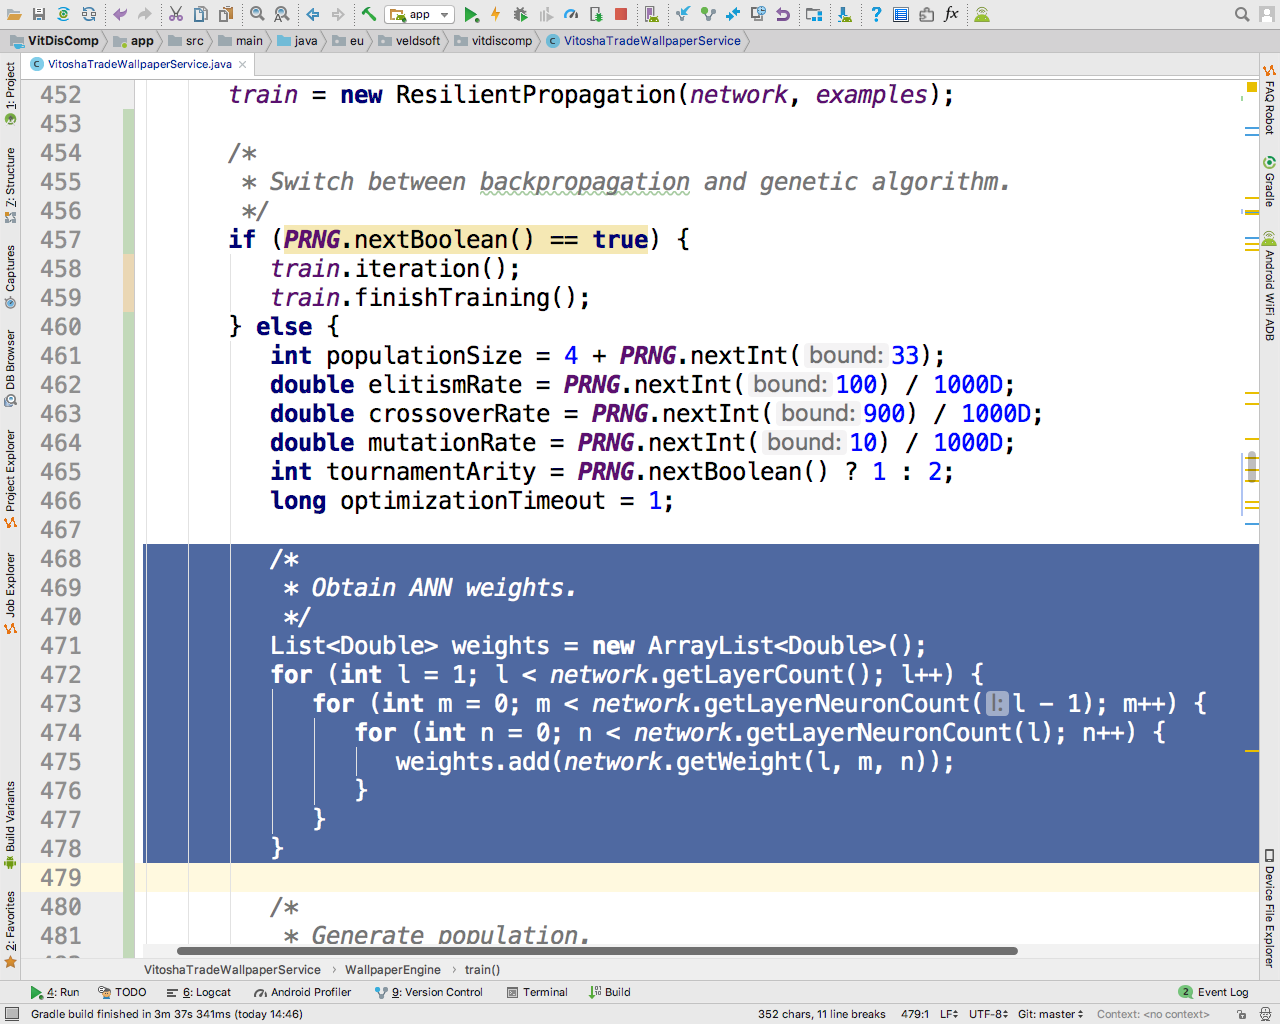
\includegraphics[height=0.45\pdfpageheight]{pic0180}
  \caption{Извличане на теглата от мрежата.}
\label{fig:pic0180}
\end{figure}
\FloatBarrier

Теглата на мрежата се подреждат във вектор от реални стойности (Фиг. \ref{fig:pic0180}).

\begin{figure}[h]
  \centering
  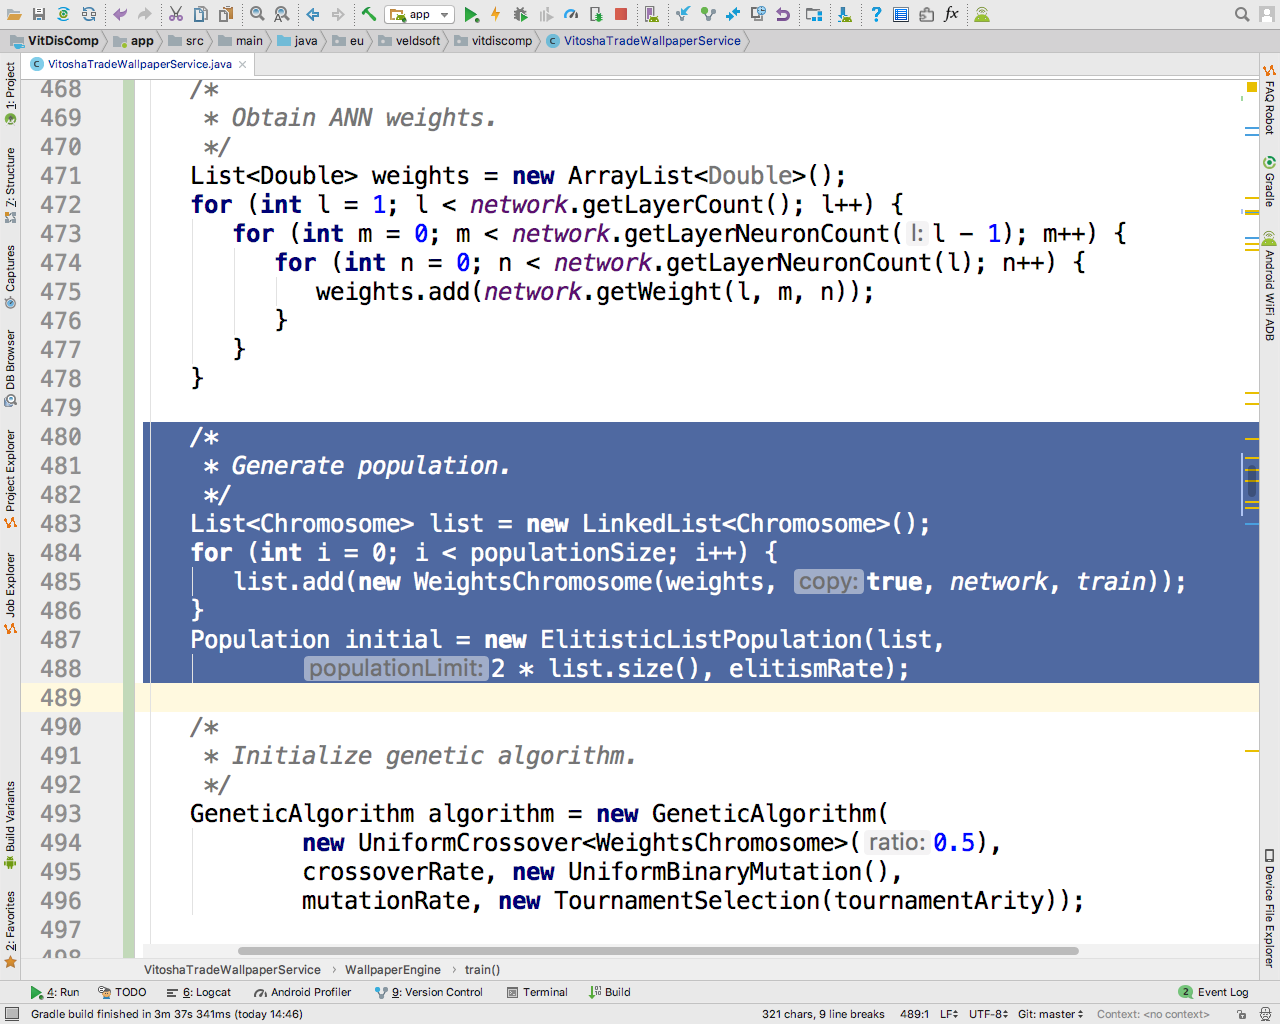
\includegraphics[height=0.45\pdfpageheight]{pic0181}
  \caption{Начална популация.}
\label{fig:pic0181}
\end{figure}
\FloatBarrier

От извлечените тегла се формира начална популация за стартиране на оптимизацията (Фиг. \ref{fig:pic0181}).

\begin{figure}[h]
  \centering
  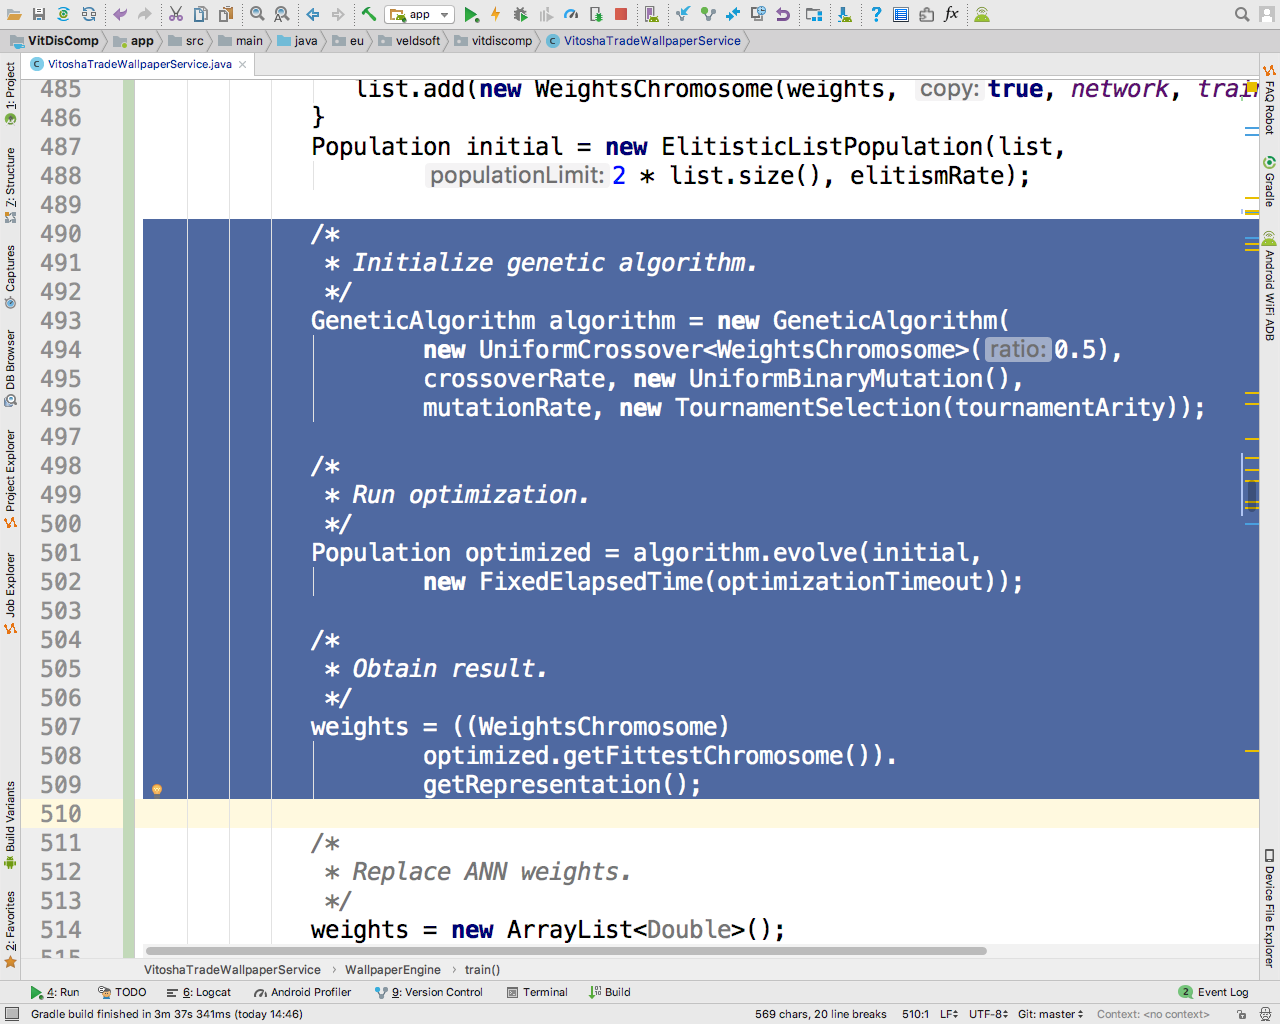
\includegraphics[height=0.45\pdfpageheight]{pic0182}
  \caption{Изпълнение на генетичния алгоритъм.}
\label{fig:pic0182}
\end{figure}
\FloatBarrier

Следва изпълнение на генетичния алгоритъм (Фиг. \ref{fig:pic0182}). За кръстосване се прилага равномерно случайно кръстосване. За мутация се прилага равномерна бинарна мутация върху всички гени на хромозомата. Най-добрият индивид от оптимизираната популация се зарежда обратно в мрежата (Фиг. \ref{fig:pic0183}). 

\begin{figure}[h]
  \centering
  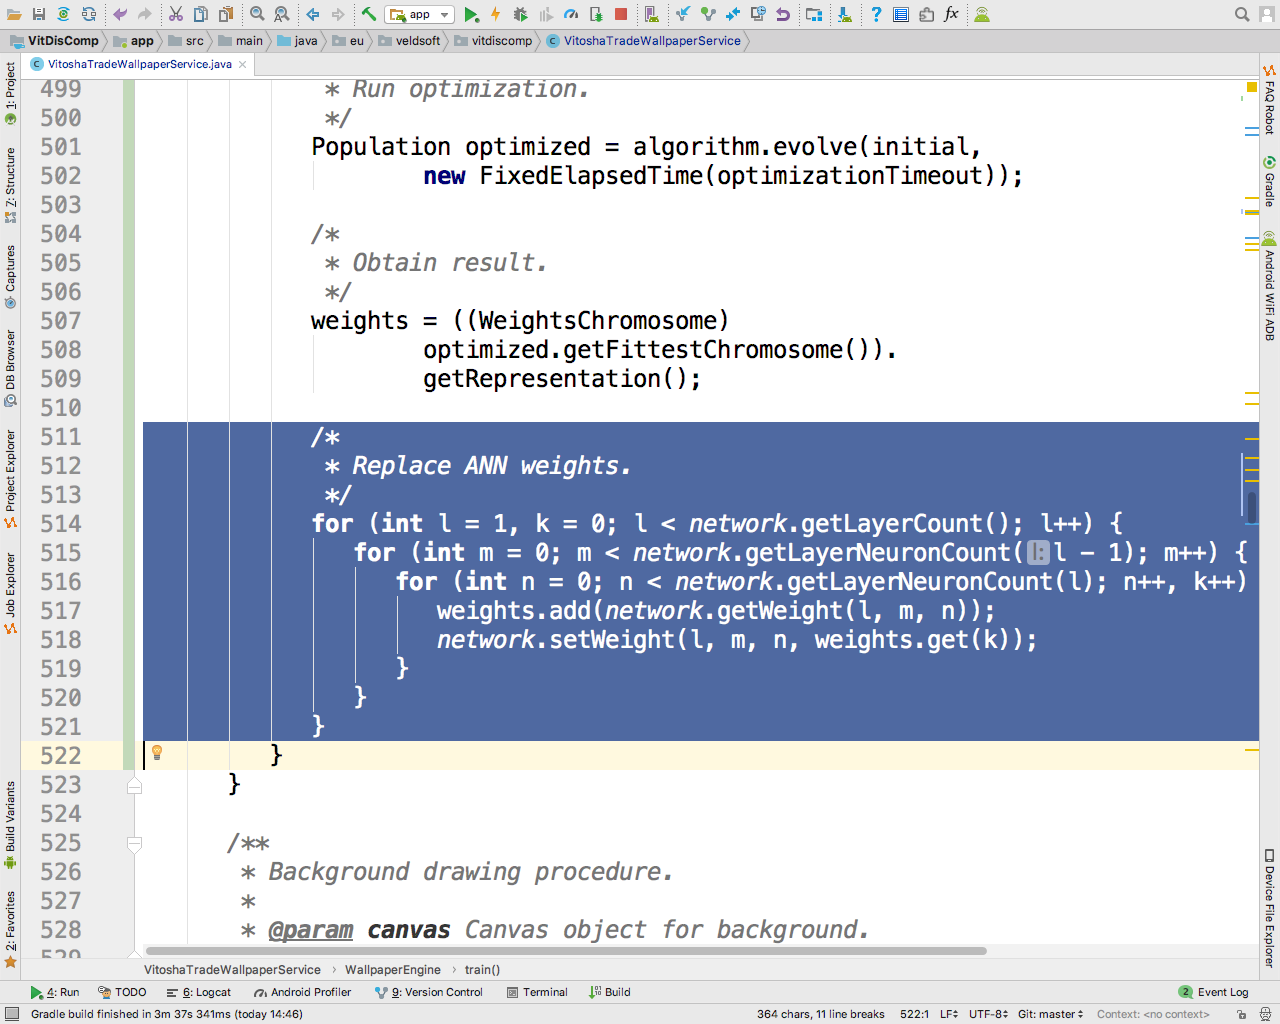
\includegraphics[height=0.45\pdfpageheight]{pic0183}
  \caption{Обновяване на теглата в мрежата.}
\label{fig:pic0183}
\end{figure}
\FloatBarrier

\subsection{Кодиране на хромозомите}

Тъй като теглата на мрежата представляват множество от реални числа, то те идеално могат да бъдат представени в хромозома съдържаща списък от стойности (Фиг. \ref{fig:pic0184}). Тъй като за оценката на жизнеността е нужно теглата да бъдат зареждани в мрежата и над мрежата да се изпълнява правия пас от обучението с обратно разпространение на грешката, то хромозомата съдържа референции към обекта за мрежа и обекта за обучение. 

\begin{figure}[h]
  \centering
  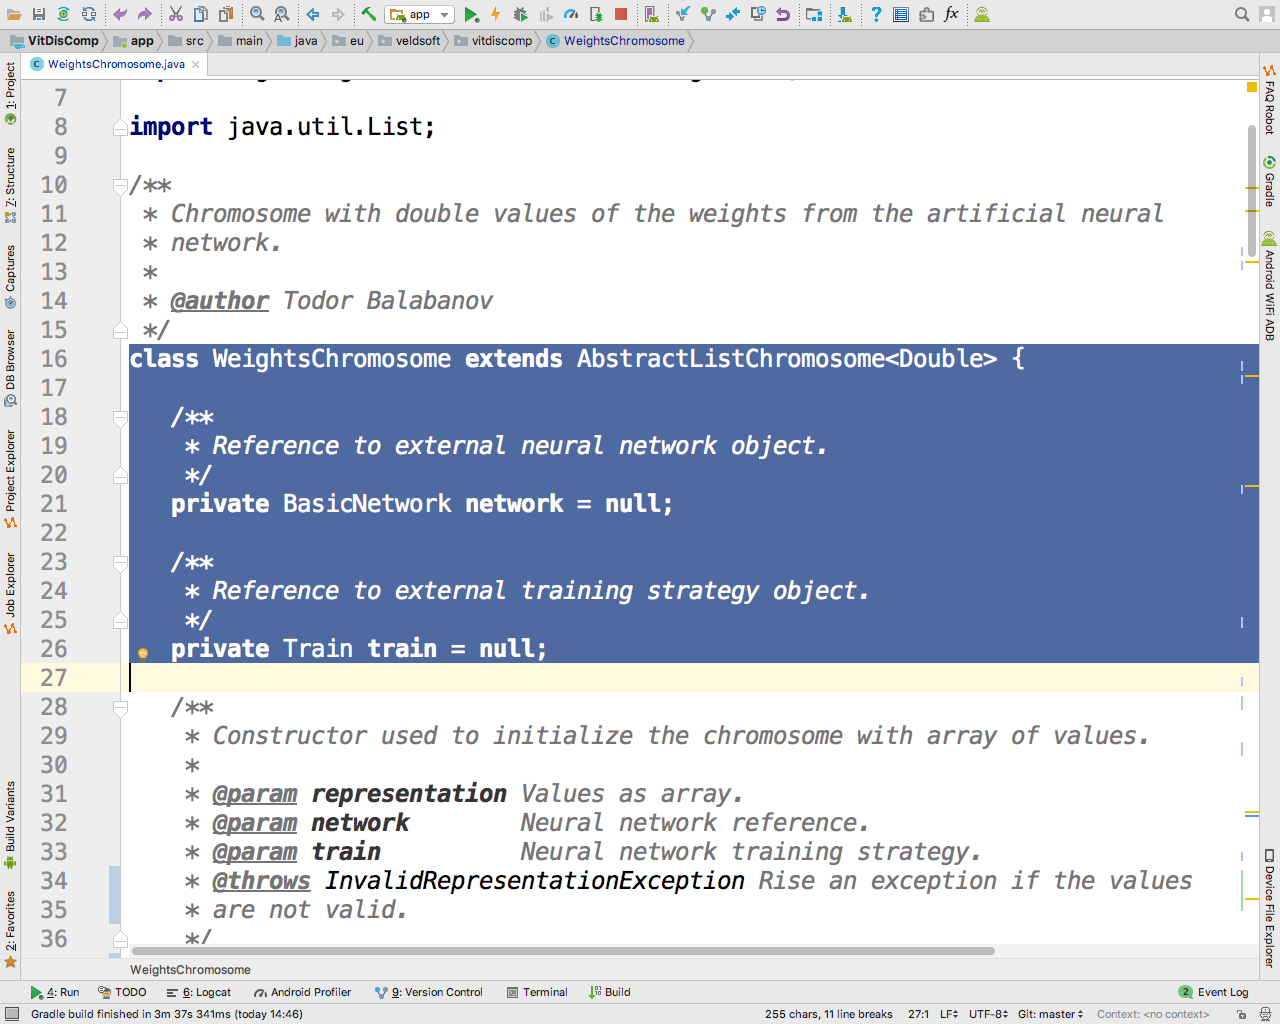
\includegraphics[height=0.45\pdfpageheight]{pic0184}
  \caption{Кодиране на теглата в хромозомите.}
\label{fig:pic0184}
\end{figure}
\FloatBarrier

За гъвкавост при създаването на обектите хромозоми са предефинирани трите наследени конструктора (Фиг. \ref{fig:pic0185}, Фиг. \ref{fig:pic0186}, Фиг. \ref{fig:pic0187}).

\begin{figure}[h]
  \centering
  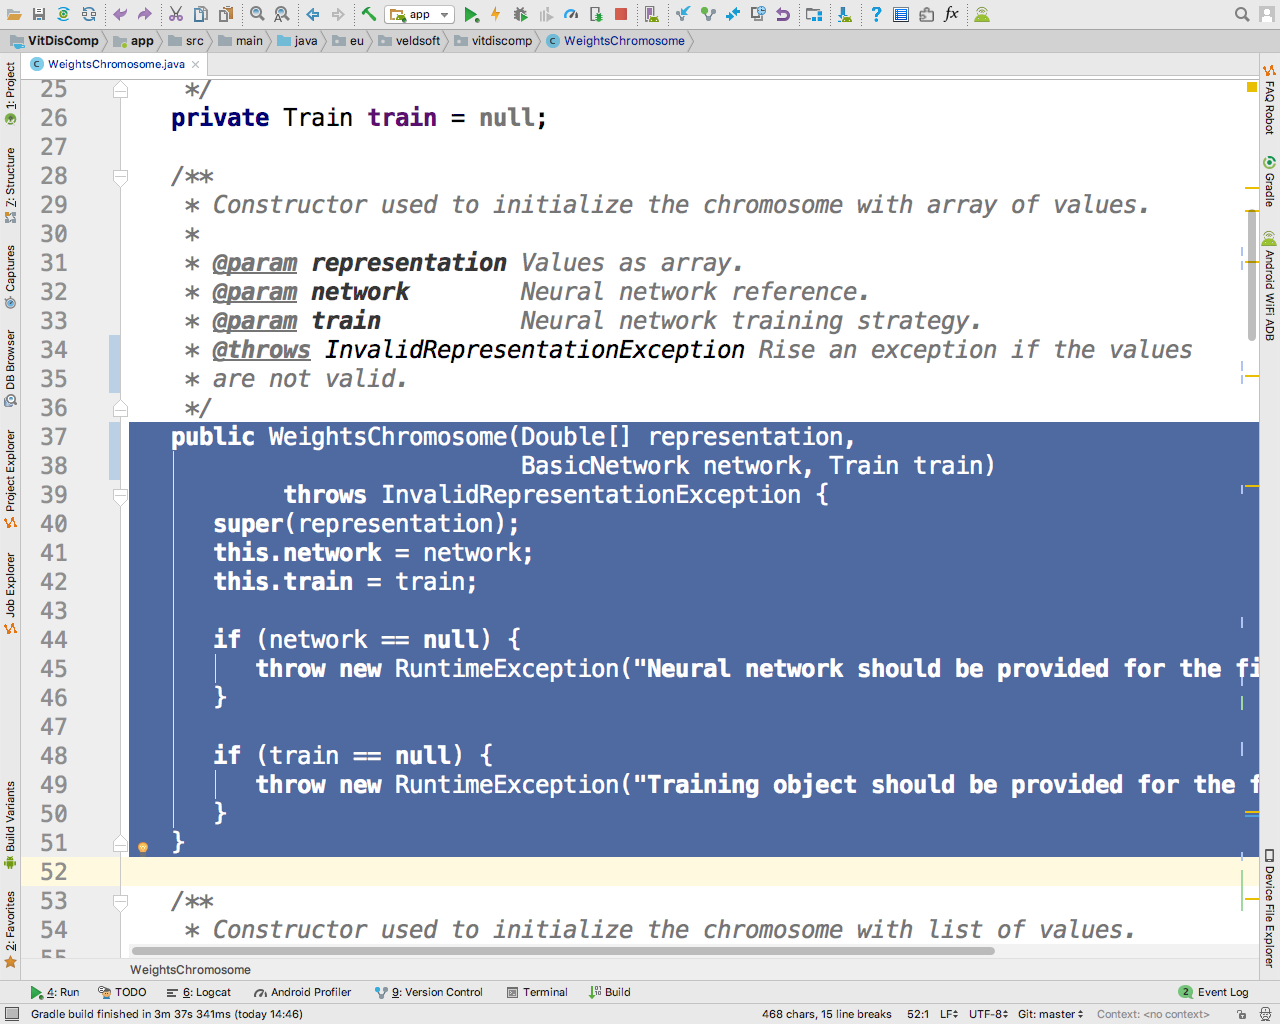
\includegraphics[height=0.45\pdfpageheight]{pic0185}
  \caption{Конструиране по зададен масив.}
\label{fig:pic0185}
\end{figure}
\FloatBarrier

\begin{figure}[h]
  \centering
  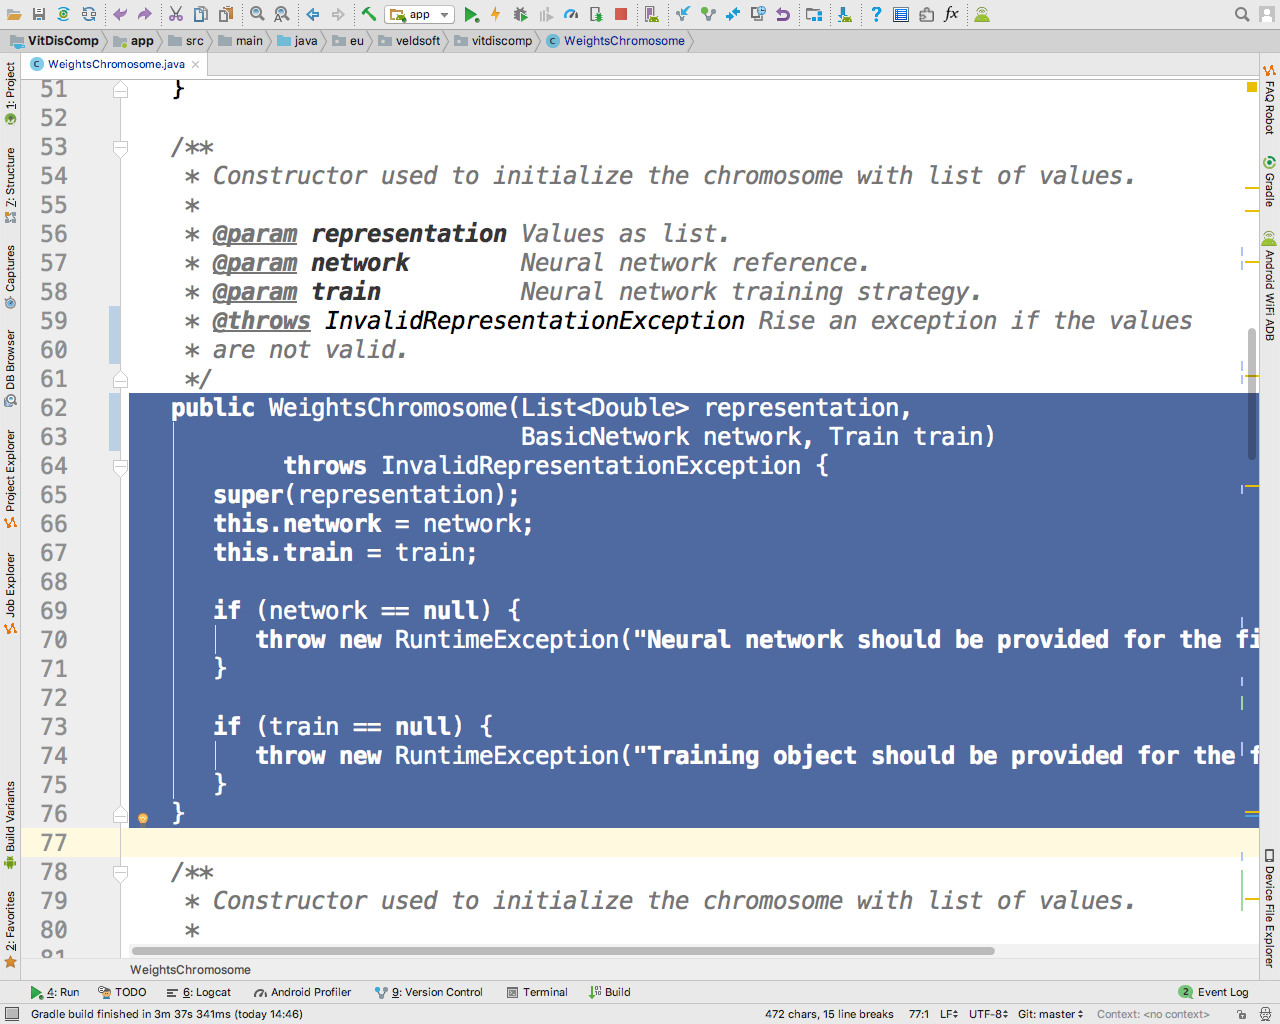
\includegraphics[height=0.45\pdfpageheight]{pic0186}
  \caption{Конструиране по зададен списък.}
\label{fig:pic0186}
\end{figure}
\FloatBarrier

\begin{figure}[h]
  \centering
  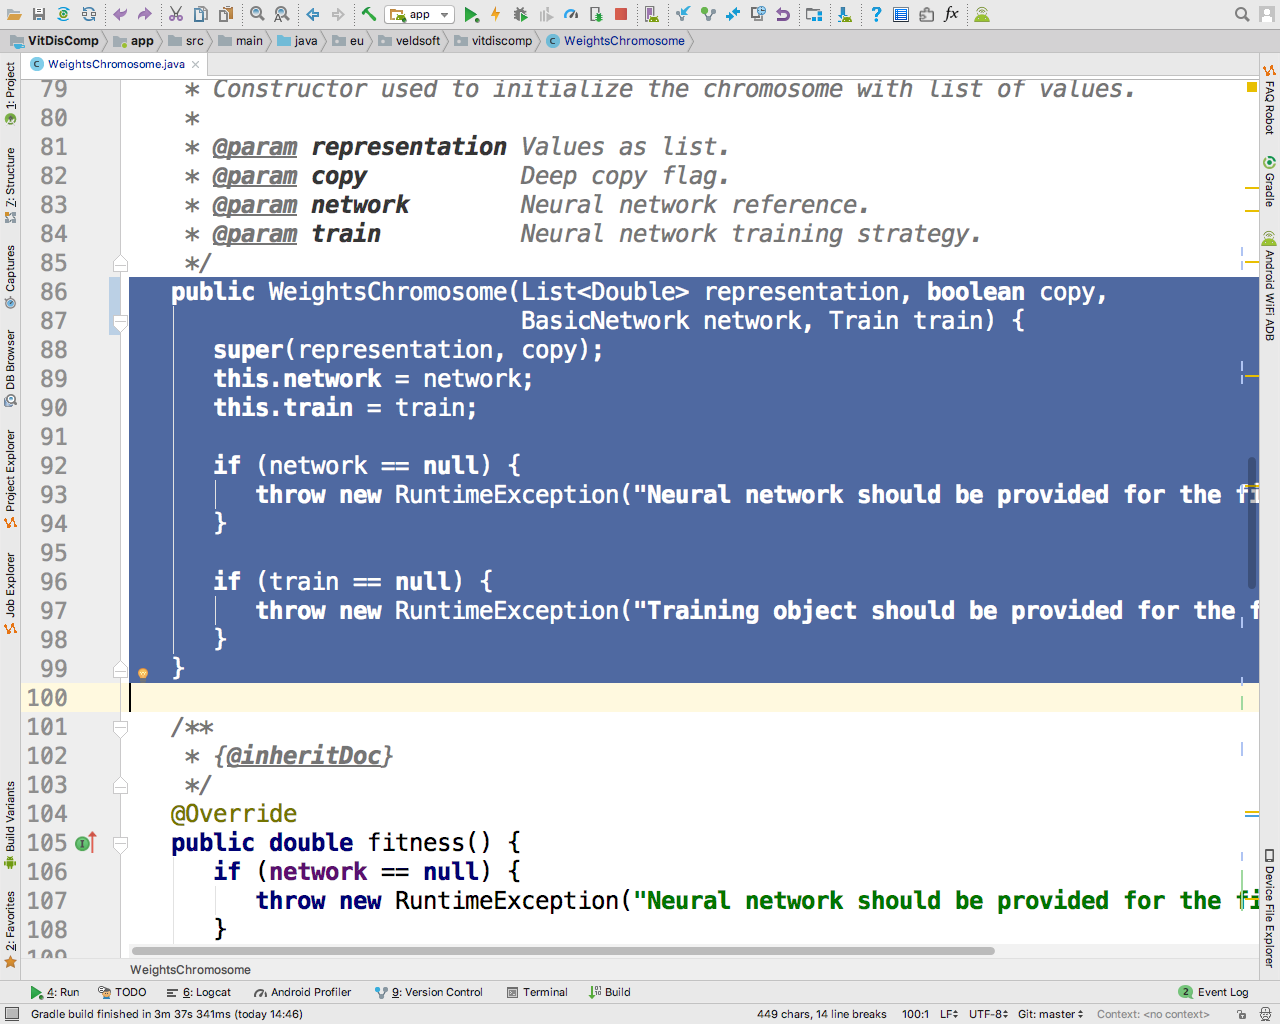
\includegraphics[height=0.45\pdfpageheight]{pic0187}
  \caption{Конструиране по зададен списък с възможност за дълбоко копиране.}
\label{fig:pic0187}
\end{figure}
\FloatBarrier

Определянето на жизнеността започва със зареждане на дробните стойности, като тегла в изкуствената невронна мрежа (Фиг. \ref{fig:pic0188}).

\begin{figure}[h]
  \centering
  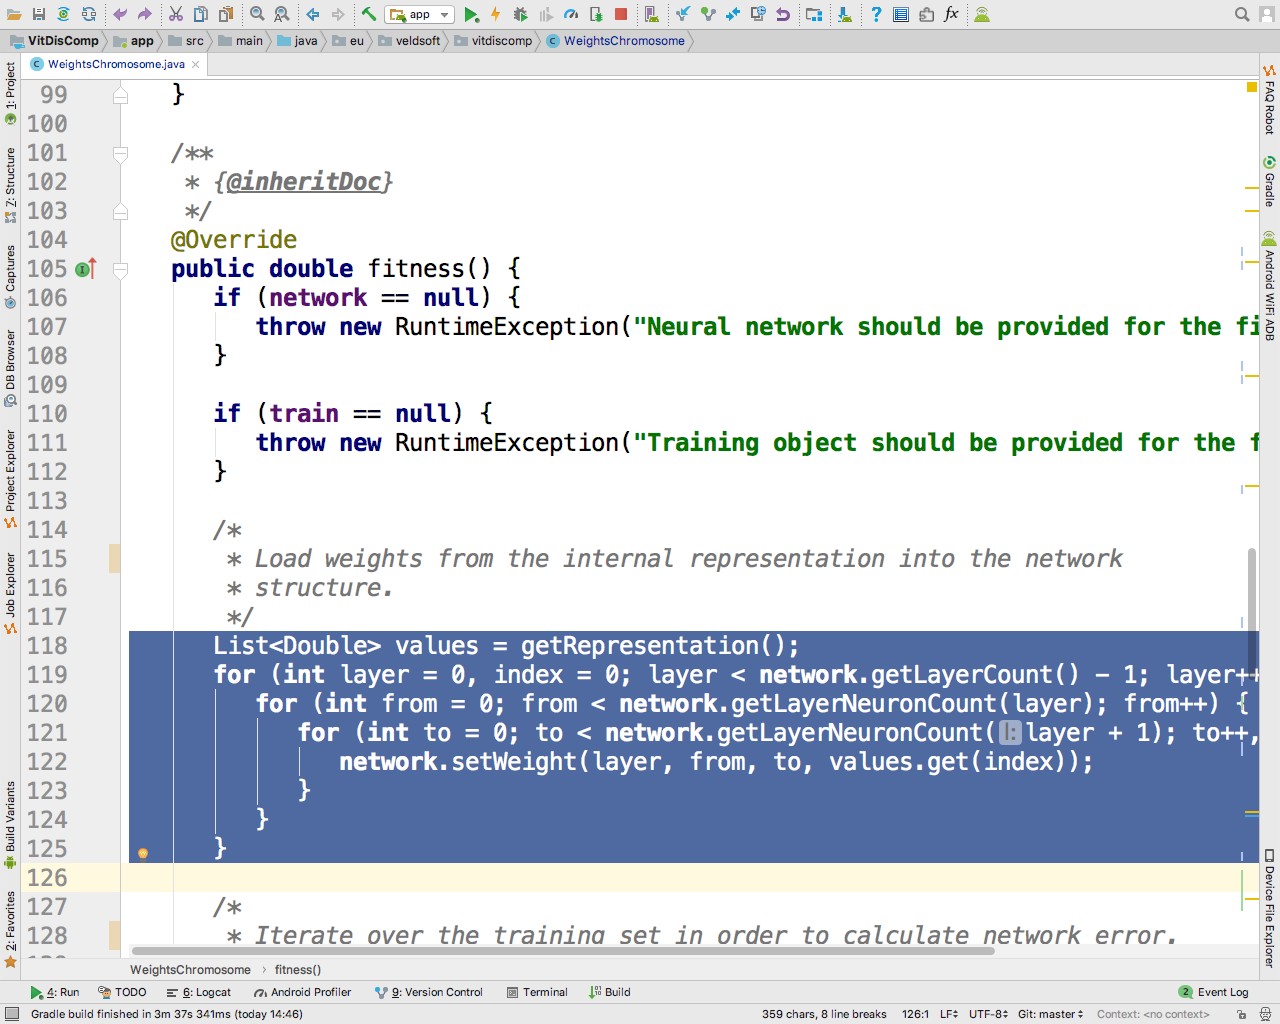
\includegraphics[height=0.45\pdfpageheight]{pic0188}
  \caption{Зареждане на стойностите като тегла в мрежата.}
\label{fig:pic0188}
\end{figure}
\FloatBarrier

Изпълнява се правия пас и общата грешка допусната от мрежата се връща като жизнена стойност (Фиг. \ref{fig:pic0189}).

\begin{figure}[h]
  \centering
  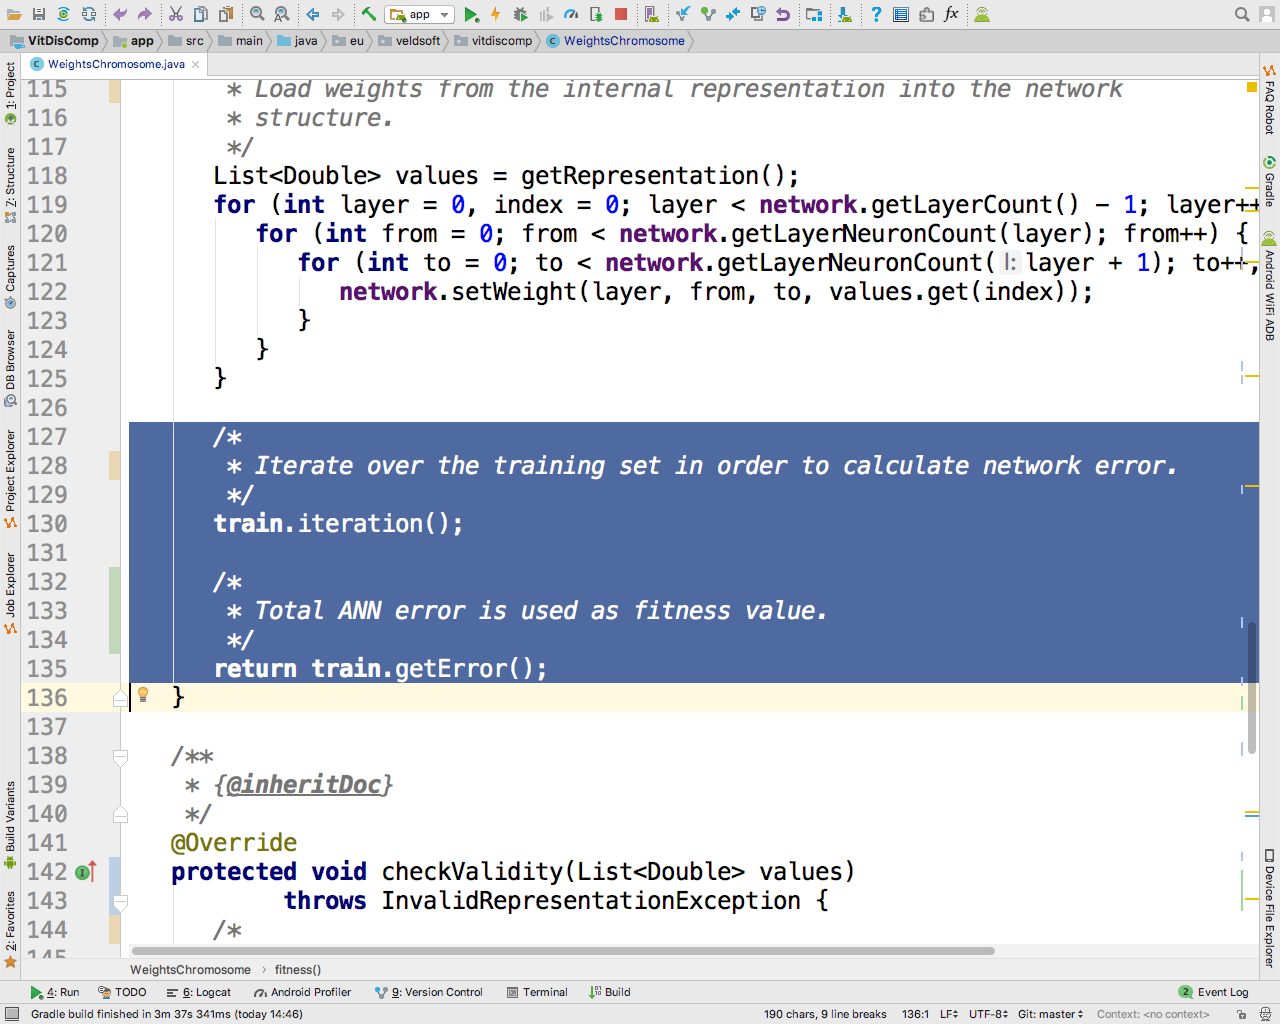
\includegraphics[height=0.45\pdfpageheight]{pic0189}
  \caption{Изпълнение на правия пас.}
\label{fig:pic0189}
\end{figure}
\FloatBarrier

Валидността на хромозомата зависи единствено от това да има достатъчно дробни числа, така че да се съпостави стойност за всяко тегло в мрежата (Фиг. \ref{fig:pic0190}).

\begin{figure}[h]
  \centering
  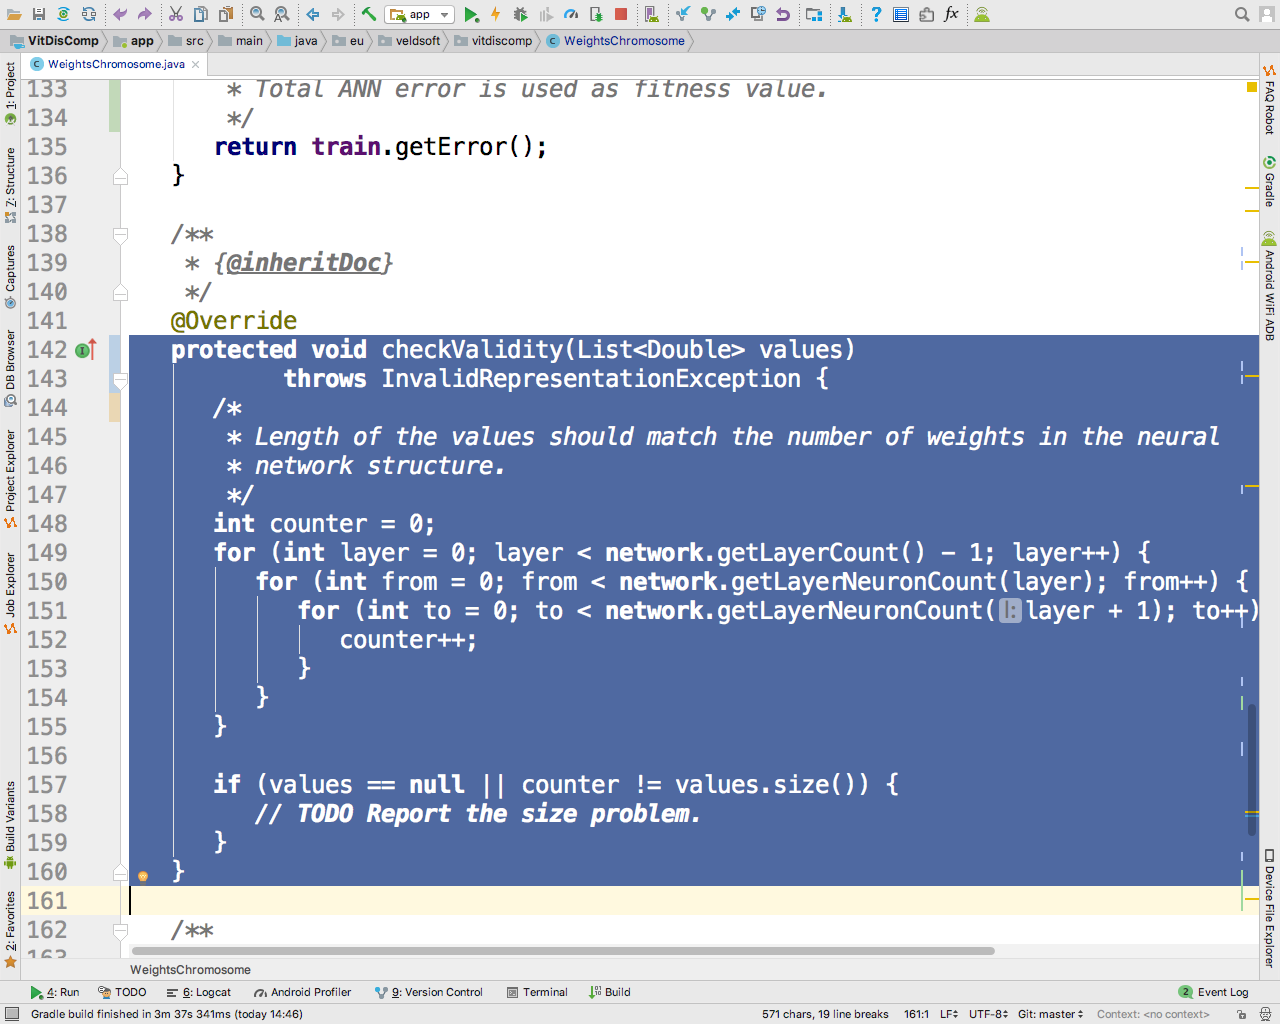
\includegraphics[height=0.45\pdfpageheight]{pic0190}
  \caption{Условие за валидност на хромозомата.}
\label{fig:pic0190}
\end{figure}
\FloatBarrier

Конструирането на нова хромозома с фиксирана дължина се извършва чрез извикването на един от конструкторите и използването на дълбоко копиране за стойностите (Фиг. \ref{fig:pic0191}).

\begin{figure}[h]
  \centering
  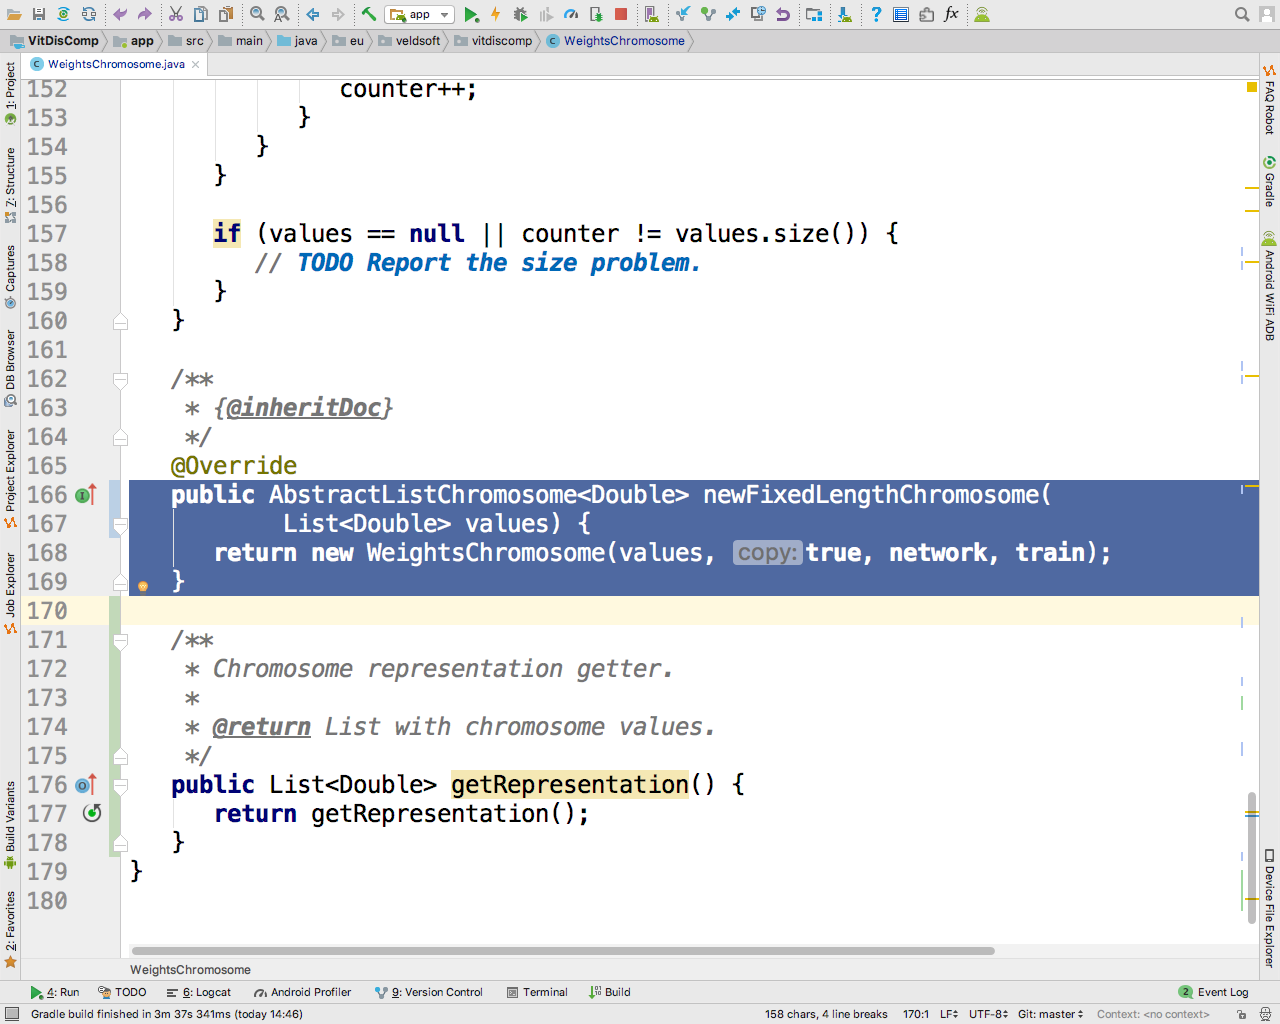
\includegraphics[height=0.45\pdfpageheight]{pic0191}
  \caption{Конструиране на нова хромозома с фиксирана дължина.}
\label{fig:pic0191}
\end{figure}
\FloatBarrier

За нуждите на пресмятанията извън класа е създадена функция за извеждане на стойностите (Фиг. \ref{fig:pic0192}).

\begin{figure}[h]
  \centering
  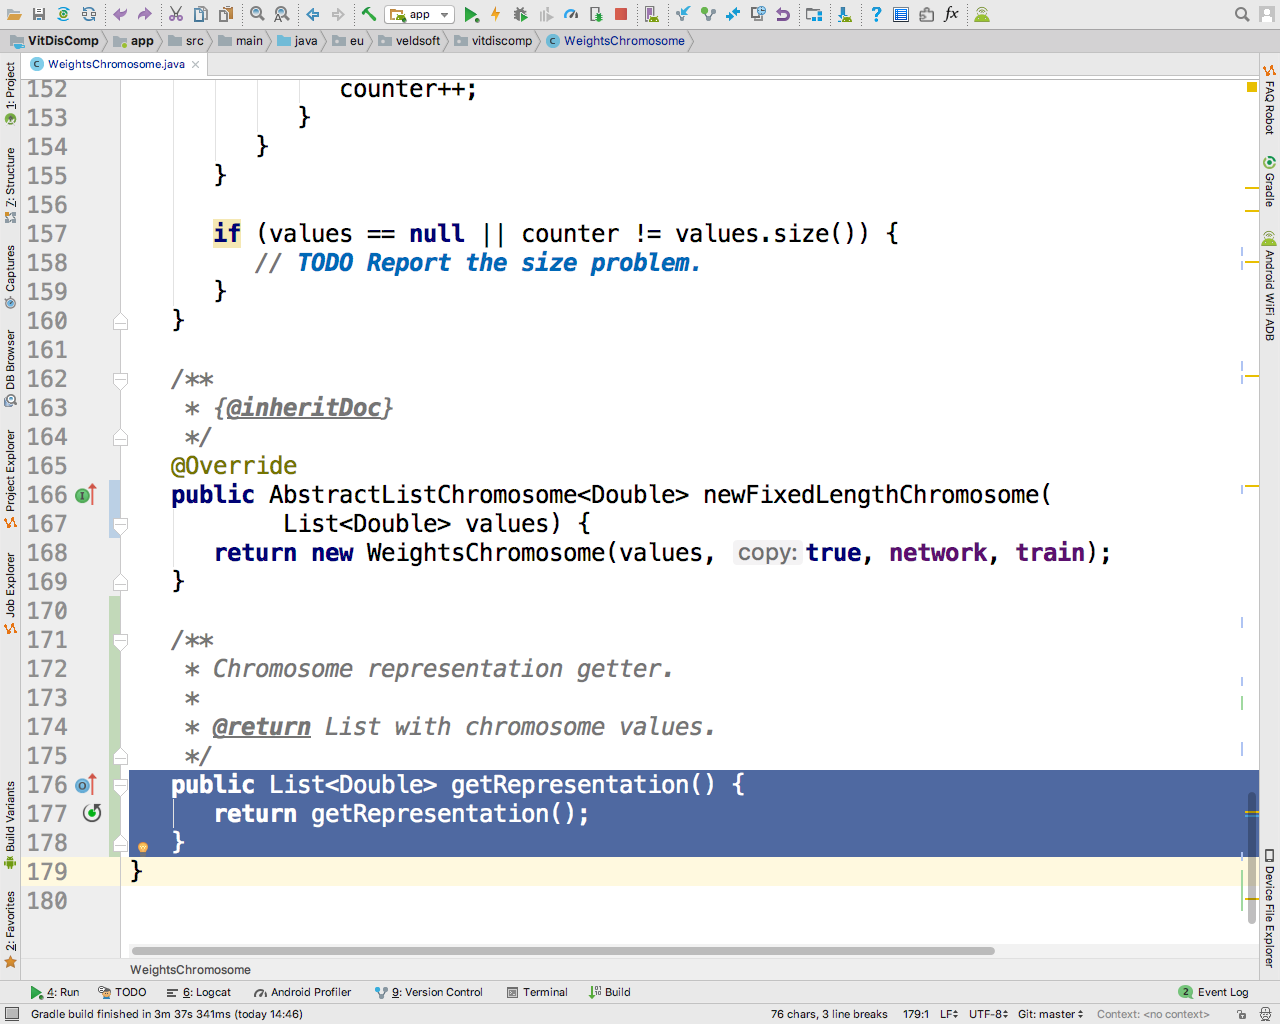
\includegraphics[height=0.45\pdfpageheight]{pic0192}
  \caption{Функция за извеждане на стойностите извън хромозомата.}
\label{fig:pic0192}
\end{figure}
\FloatBarrier

\subsection{Случайна равномерна мутация}

Тъй като библиотеката Genetic Algorithms - Apache Commons не предлага подходяща бинарна мутация за вектор от реални числа, то за нуждите на разработката е предложен клас изпълняващ операцията по мутация (Фиг. ).

\begin{figure}[h]
  \centering
  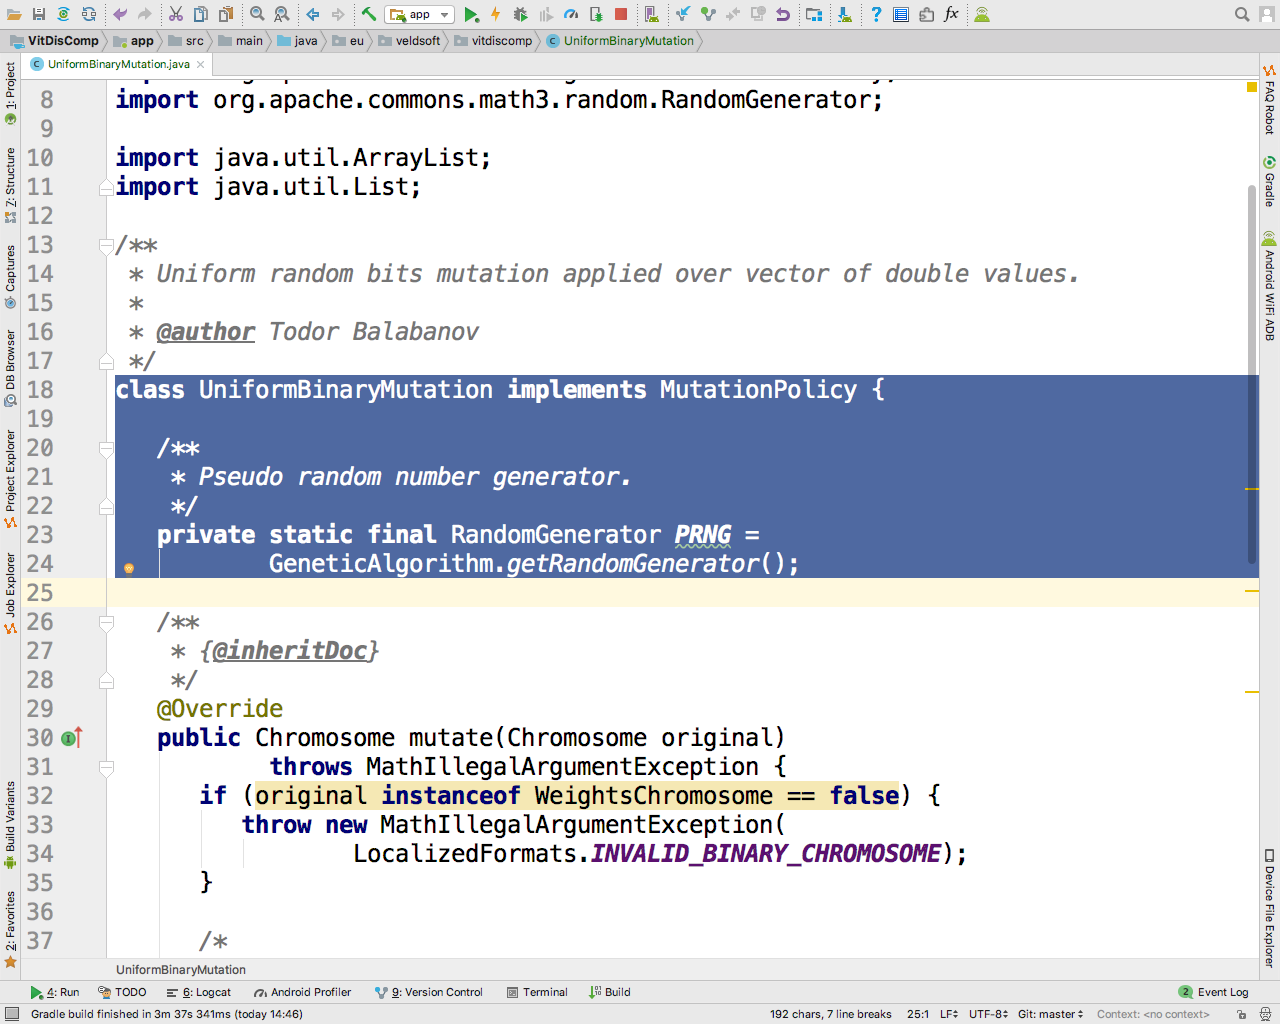
\includegraphics[height=0.45\pdfpageheight]{pic0193}
  \caption{Клас извършващ мутацията.}
\label{fig:pic0193}
\end{figure}
\FloatBarrier

Предложената операция за мутация е удачно да се прилага само върху използваното кодиране в хромозомите. Поради тази причина функцията за мутация извършва нужната проверка на входните данни (Фиг. \ref{fig:pic0194}).

\begin{figure}[h]
  \centering
  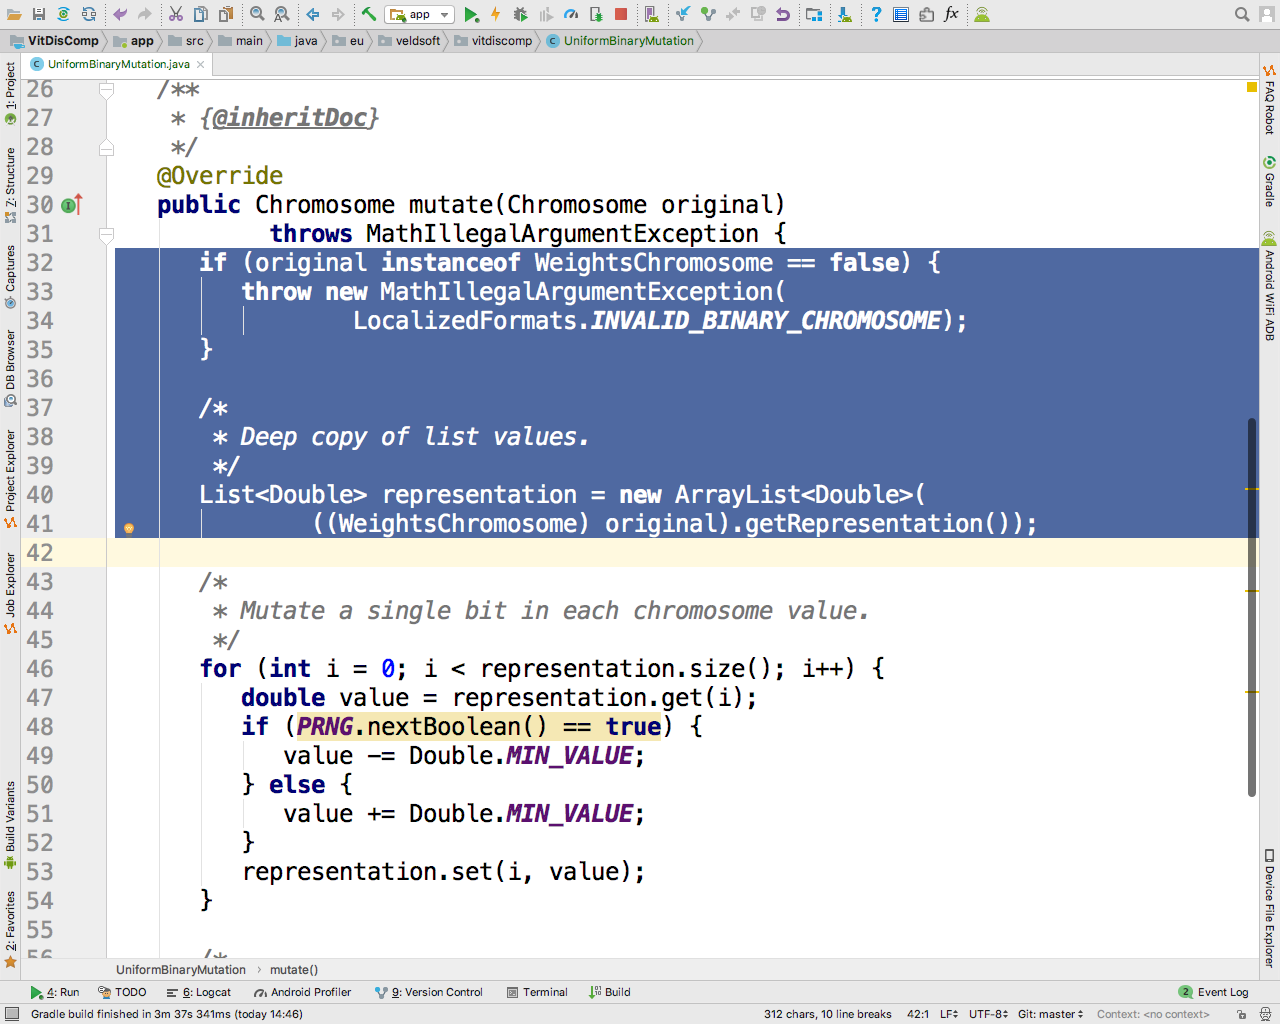
\includegraphics[height=0.45\pdfpageheight]{pic0194}
  \caption{Контрол на входните данни.}
\label{fig:pic0194}
\end{figure}
\FloatBarrier

За разлика от класическата мутация в генетичните алгоритми, при тази разработка е направена модификация, наподобяваща метода за еволюция на разликите. Всеки ген в хромозомата бива променен с малка дробна стойност (Фиг. \ref{fig:pic0195}). 

\begin{figure}[h]
  \centering
  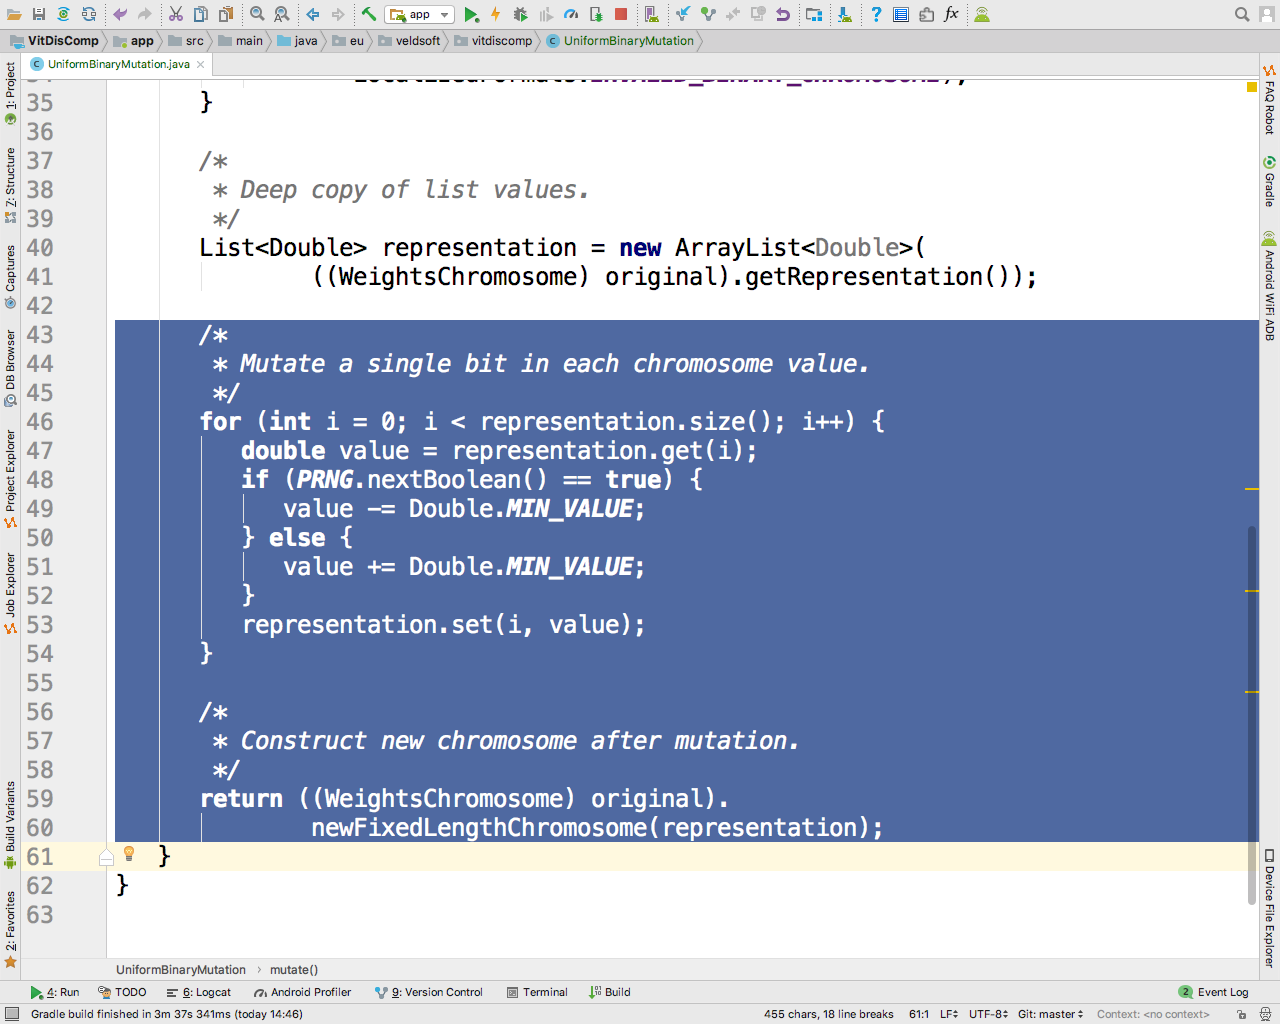
\includegraphics[height=0.45\pdfpageheight]{pic0195}
  \caption{Случайна промяна на всички стойности в хромозомата.}
\label{fig:pic0195}
\end{figure}
\FloatBarrier

Мутацията приключва със създаване и връщане на мутирал екземпляр.
